% Left: Euler's gamma as the area between the bars 1/k and the curve 1/t. Right: partial sums of rearrangements of the alternating harmonic series. Generated by a short script (numpy).
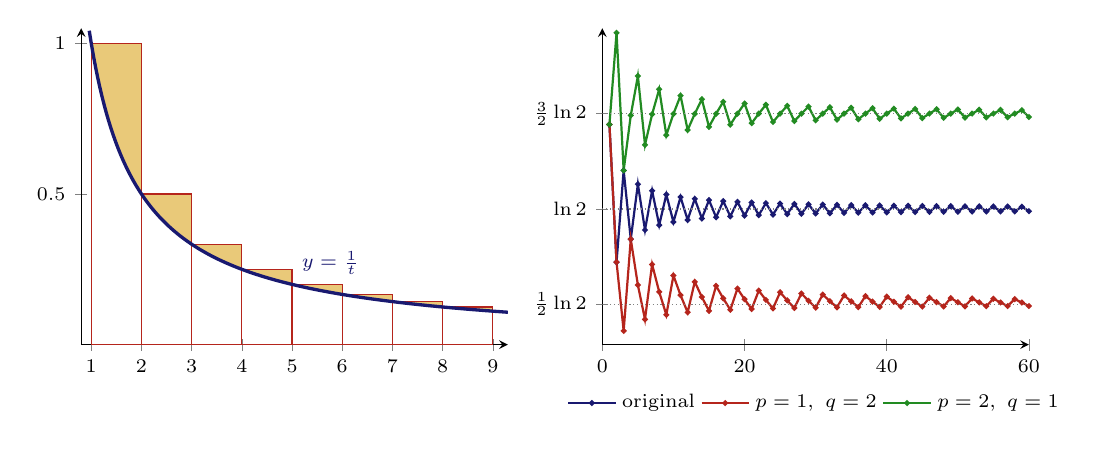
\begin{tikzpicture}
\begin{axis}[name=L,width=7cm,height=5.6cm,xmin=0.8,xmax=9.3,ymin=0,ymax=1.05,axis lines=left,xtick={1,...,9},ytick={0.5,1},tick label style={font=\scriptsize}]
\addplot[fill=Goldenrod!60,draw=none] coordinates {(1,1.0000) (2,1.0000) (2.0000,0.5000) (1.9655,0.5088) (1.9310,0.5179) (1.8966,0.5273) (1.8621,0.5370) (1.8276,0.5472) (1.7931,0.5577) (1.7586,0.5686) (1.7241,0.5800) (1.6897,0.5918) (1.6552,0.6042) (1.6207,0.6170) (1.5862,0.6304) (1.5517,0.6444) (1.5172,0.6591) (1.4828,0.6744) (1.4483,0.6905) (1.4138,0.7073) (1.3793,0.7250) (1.3448,0.7436) (1.3103,0.7632) (1.2759,0.7838) (1.2414,0.8056) (1.2069,0.8286) (1.1724,0.8529) (1.1379,0.8788) (1.1034,0.9062) (1.0690,0.9355) (1.0345,0.9667) (1.0000,1.0000)} -- cycle;
\draw[BrickRed] (axis cs:1,0) rectangle (axis cs:2,1.0000);
\addplot[fill=Goldenrod!60,draw=none] coordinates {(2,0.5000) (3,0.5000) (3.0000,0.3333) (2.9655,0.3372) (2.9310,0.3412) (2.8966,0.3452) (2.8621,0.3494) (2.8276,0.3537) (2.7931,0.3580) (2.7586,0.3625) (2.7241,0.3671) (2.6897,0.3718) (2.6552,0.3766) (2.6207,0.3816) (2.5862,0.3867) (2.5517,0.3919) (2.5172,0.3973) (2.4828,0.4028) (2.4483,0.4085) (2.4138,0.4143) (2.3793,0.4203) (2.3448,0.4265) (2.3103,0.4328) (2.2759,0.4394) (2.2414,0.4462) (2.2069,0.4531) (2.1724,0.4603) (2.1379,0.4677) (2.1034,0.4754) (2.0690,0.4833) (2.0345,0.4915) (2.0000,0.5000)} -- cycle;
\draw[BrickRed] (axis cs:2,0) rectangle (axis cs:3,0.5000);
\addplot[fill=Goldenrod!60,draw=none] coordinates {(3,0.3333) (4,0.3333) (4.0000,0.2500) (3.9655,0.2522) (3.9310,0.2544) (3.8966,0.2566) (3.8621,0.2589) (3.8276,0.2613) (3.7931,0.2636) (3.7586,0.2661) (3.7241,0.2685) (3.6897,0.2710) (3.6552,0.2736) (3.6207,0.2762) (3.5862,0.2788) (3.5517,0.2816) (3.5172,0.2843) (3.4828,0.2871) (3.4483,0.2900) (3.4138,0.2929) (3.3793,0.2959) (3.3448,0.2990) (3.3103,0.3021) (3.2759,0.3053) (3.2414,0.3085) (3.2069,0.3118) (3.1724,0.3152) (3.1379,0.3187) (3.1034,0.3222) (3.0690,0.3258) (3.0345,0.3295) (3.0000,0.3333)} -- cycle;
\draw[BrickRed] (axis cs:3,0) rectangle (axis cs:4,0.3333);
\addplot[fill=Goldenrod!60,draw=none] coordinates {(4,0.2500) (5,0.2500) (5.0000,0.2000) (4.9655,0.2014) (4.9310,0.2028) (4.8966,0.2042) (4.8621,0.2057) (4.8276,0.2071) (4.7931,0.2086) (4.7586,0.2101) (4.7241,0.2117) (4.6897,0.2132) (4.6552,0.2148) (4.6207,0.2164) (4.5862,0.2180) (4.5517,0.2197) (4.5172,0.2214) (4.4828,0.2231) (4.4483,0.2248) (4.4138,0.2266) (4.3793,0.2283) (4.3448,0.2302) (4.3103,0.2320) (4.2759,0.2339) (4.2414,0.2358) (4.2069,0.2377) (4.1724,0.2397) (4.1379,0.2417) (4.1034,0.2437) (4.0690,0.2458) (4.0345,0.2479) (4.0000,0.2500)} -- cycle;
\draw[BrickRed] (axis cs:4,0) rectangle (axis cs:5,0.2500);
\addplot[fill=Goldenrod!60,draw=none] coordinates {(5,0.2000) (6,0.2000) (6.0000,0.1667) (5.9655,0.1676) (5.9310,0.1686) (5.8966,0.1696) (5.8621,0.1706) (5.8276,0.1716) (5.7931,0.1726) (5.7586,0.1737) (5.7241,0.1747) (5.6897,0.1758) (5.6552,0.1768) (5.6207,0.1779) (5.5862,0.1790) (5.5517,0.1801) (5.5172,0.1812) (5.4828,0.1824) (5.4483,0.1835) (5.4138,0.1847) (5.3793,0.1859) (5.3448,0.1871) (5.3103,0.1883) (5.2759,0.1895) (5.2414,0.1908) (5.2069,0.1921) (5.1724,0.1933) (5.1379,0.1946) (5.1034,0.1959) (5.0690,0.1973) (5.0345,0.1986) (5.0000,0.2000)} -- cycle;
\draw[BrickRed] (axis cs:5,0) rectangle (axis cs:6,0.2000);
\addplot[fill=Goldenrod!60,draw=none] coordinates {(6,0.1667) (7,0.1667) (7.0000,0.1429) (6.9655,0.1436) (6.9310,0.1443) (6.8966,0.1450) (6.8621,0.1457) (6.8276,0.1465) (6.7931,0.1472) (6.7586,0.1480) (6.7241,0.1487) (6.6897,0.1495) (6.6552,0.1503) (6.6207,0.1510) (6.5862,0.1518) (6.5517,0.1526) (6.5172,0.1534) (6.4828,0.1543) (6.4483,0.1551) (6.4138,0.1559) (6.3793,0.1568) (6.3448,0.1576) (6.3103,0.1585) (6.2759,0.1593) (6.2414,0.1602) (6.2069,0.1611) (6.1724,0.1620) (6.1379,0.1629) (6.1034,0.1638) (6.0690,0.1648) (6.0345,0.1657) (6.0000,0.1667)} -- cycle;
\draw[BrickRed] (axis cs:6,0) rectangle (axis cs:7,0.1667);
\addplot[fill=Goldenrod!60,draw=none] coordinates {(7,0.1429) (8,0.1429) (8.0000,0.1250) (7.9655,0.1255) (7.9310,0.1261) (7.8966,0.1266) (7.8621,0.1272) (7.8276,0.1278) (7.7931,0.1283) (7.7586,0.1289) (7.7241,0.1295) (7.6897,0.1300) (7.6552,0.1306) (7.6207,0.1312) (7.5862,0.1318) (7.5517,0.1324) (7.5172,0.1330) (7.4828,0.1336) (7.4483,0.1343) (7.4138,0.1349) (7.3793,0.1355) (7.3448,0.1362) (7.3103,0.1368) (7.2759,0.1374) (7.2414,0.1381) (7.2069,0.1388) (7.1724,0.1394) (7.1379,0.1401) (7.1034,0.1408) (7.0690,0.1415) (7.0345,0.1422) (7.0000,0.1429)} -- cycle;
\draw[BrickRed] (axis cs:7,0) rectangle (axis cs:8,0.1429);
\addplot[fill=Goldenrod!60,draw=none] coordinates {(8,0.1250) (9,0.1250) (9.0000,0.1111) (8.9655,0.1115) (8.9310,0.1120) (8.8966,0.1124) (8.8621,0.1128) (8.8276,0.1133) (8.7931,0.1137) (8.7586,0.1142) (8.7241,0.1146) (8.6897,0.1151) (8.6552,0.1155) (8.6207,0.1160) (8.5862,0.1165) (8.5517,0.1169) (8.5172,0.1174) (8.4828,0.1179) (8.4483,0.1184) (8.4138,0.1189) (8.3793,0.1193) (8.3448,0.1198) (8.3103,0.1203) (8.2759,0.1208) (8.2414,0.1213) (8.2069,0.1218) (8.1724,0.1224) (8.1379,0.1229) (8.1034,0.1234) (8.0690,0.1239) (8.0345,0.1245) (8.0000,0.1250)} -- cycle;
\draw[BrickRed] (axis cs:8,0) rectangle (axis cs:9,0.1250);
\addplot[MidnightBlue,very thick] coordinates {(0.9600,1.0417) (1.0019,0.9981) (1.0438,0.9580) (1.0857,0.9210) (1.1276,0.8868) (1.1695,0.8550) (1.2115,0.8255) (1.2534,0.7979) (1.2953,0.7720) (1.3372,0.7478) (1.3791,0.7251) (1.4210,0.7037) (1.4629,0.6836) (1.5048,0.6645) (1.5467,0.6465) (1.5886,0.6295) (1.6306,0.6133) (1.6725,0.5979) (1.7144,0.5833) (1.7563,0.5694) (1.7982,0.5561) (1.8401,0.5434) (1.8820,0.5313) (1.9239,0.5198) (1.9658,0.5087) (2.0077,0.4981) (2.0496,0.4879) (2.0916,0.4781) (2.1335,0.4687) (2.1754,0.4597) (2.2173,0.4510) (2.2592,0.4426) (2.3011,0.4346) (2.3430,0.4268) (2.3849,0.4193) (2.4268,0.4121) (2.4687,0.4051) (2.5107,0.3983) (2.5526,0.3918) (2.5945,0.3854) (2.6364,0.3793) (2.6783,0.3734) (2.7202,0.3676) (2.7621,0.3620) (2.8040,0.3566) (2.8459,0.3514) (2.8878,0.3463) (2.9297,0.3413) (2.9717,0.3365) (3.0136,0.3318) (3.0555,0.3273) (3.0974,0.3229) (3.1393,0.3185) (3.1812,0.3143) (3.2231,0.3103) (3.2650,0.3063) (3.3069,0.3024) (3.3488,0.2986) (3.3908,0.2949) (3.4327,0.2913) (3.4746,0.2878) (3.5165,0.2844) (3.5584,0.2810) (3.6003,0.2778) (3.6422,0.2746) (3.6841,0.2714) (3.7260,0.2684) (3.7679,0.2654) (3.8098,0.2625) (3.8518,0.2596) (3.8937,0.2568) (3.9356,0.2541) (3.9775,0.2514) (4.0194,0.2488) (4.0613,0.2462) (4.1032,0.2437) (4.1451,0.2412) (4.1870,0.2388) (4.2289,0.2365) (4.2709,0.2341) (4.3128,0.2319) (4.3547,0.2296) (4.3966,0.2274) (4.4385,0.2253) (4.4804,0.2232) (4.5223,0.2211) (4.5642,0.2191) (4.6061,0.2171) (4.6480,0.2151) (4.6899,0.2132) (4.7319,0.2113) (4.7738,0.2095) (4.8157,0.2077) (4.8576,0.2059) (4.8995,0.2041) (4.9414,0.2024) (4.9833,0.2007) (5.0252,0.1990) (5.0671,0.1974) (5.1090,0.1957) (5.1510,0.1941) (5.1929,0.1926) (5.2348,0.1910) (5.2767,0.1895) (5.3186,0.1880) (5.3605,0.1865) (5.4024,0.1851) (5.4443,0.1837) (5.4862,0.1823) (5.5281,0.1809) (5.5701,0.1795) (5.6120,0.1782) (5.6539,0.1769) (5.6958,0.1756) (5.7377,0.1743) (5.7796,0.1730) (5.8215,0.1718) (5.8634,0.1705) (5.9053,0.1693) (5.9472,0.1681) (5.9891,0.1670) (6.0311,0.1658) (6.0730,0.1647) (6.1149,0.1635) (6.1568,0.1624) (6.1987,0.1613) (6.2406,0.1602) (6.2825,0.1592) (6.3244,0.1581) (6.3663,0.1571) (6.4082,0.1560) (6.4502,0.1550) (6.4921,0.1540) (6.5340,0.1530) (6.5759,0.1521) (6.6178,0.1511) (6.6597,0.1502) (6.7016,0.1492) (6.7435,0.1483) (6.7854,0.1474) (6.8273,0.1465) (6.8692,0.1456) (6.9112,0.1447) (6.9531,0.1438) (6.9950,0.1430) (7.0369,0.1421) (7.0788,0.1413) (7.1207,0.1404) (7.1626,0.1396) (7.2045,0.1388) (7.2464,0.1380) (7.2883,0.1372) (7.3303,0.1364) (7.3722,0.1356) (7.4141,0.1349) (7.4560,0.1341) (7.4979,0.1334) (7.5398,0.1326) (7.5817,0.1319) (7.6236,0.1312) (7.6655,0.1305) (7.7074,0.1297) (7.7493,0.1290) (7.7913,0.1283) (7.8332,0.1277) (7.8751,0.1270) (7.9170,0.1263) (7.9589,0.1256) (8.0008,0.1250) (8.0427,0.1243) (8.0846,0.1237) (8.1265,0.1231) (8.1684,0.1224) (8.2104,0.1218) (8.2523,0.1212) (8.2942,0.1206) (8.3361,0.1200) (8.3780,0.1194) (8.4199,0.1188) (8.4618,0.1182) (8.5037,0.1176) (8.5456,0.1170) (8.5875,0.1164) (8.6294,0.1159) (8.6714,0.1153) (8.7133,0.1148) (8.7552,0.1142) (8.7971,0.1137) (8.8390,0.1131) (8.8809,0.1126) (8.9228,0.1121) (8.9647,0.1115) (9.0066,0.1110) (9.0485,0.1105) (9.0905,0.1100) (9.1324,0.1095) (9.1743,0.1090) (9.2162,0.1085) (9.2581,0.1080) (9.3000,0.1075)};
\node[font=\scriptsize,MidnightBlue,anchor=south west] at (axis cs:5,0.2) {$y=\frac1t$};
\end{axis}
\begin{axis}[at={(L.east)},anchor=west,xshift=1.2cm,width=7cm,height=5.6cm,xmin=0,xmax=60,ymin=0.2,ymax=1.35,axis lines=left,xtick={0,20,40,60},ytick={0.3466,0.6931,1.0397},yticklabels={$\frac12\ln2$,$\ln2$,$\frac32\ln2$},tick label style={font=\scriptsize},legend style={font=\scriptsize,at={(0.5,-0.12)},anchor=north,legend columns=3,draw=none}]
\addplot[MidnightBlue,thick,mark=*,mark size=0.6pt] coordinates {(1.0000,1.0000) (2.0000,0.5000) (3.0000,0.8333) (4.0000,0.5833) (5.0000,0.7833) (6.0000,0.6167) (7.0000,0.7595) (8.0000,0.6345) (9.0000,0.7456) (10.0000,0.6456) (11.0000,0.7365) (12.0000,0.6532) (13.0000,0.7301) (14.0000,0.6587) (15.0000,0.7254) (16.0000,0.6629) (17.0000,0.7217) (18.0000,0.6661) (19.0000,0.7188) (20.0000,0.6688) (21.0000,0.7164) (22.0000,0.6709) (23.0000,0.7144) (24.0000,0.6727) (25.0000,0.7127) (26.0000,0.6743) (27.0000,0.7113) (28.0000,0.6756) (29.0000,0.7101) (30.0000,0.6768) (31.0000,0.7090) (32.0000,0.6778) (33.0000,0.7081) (34.0000,0.6787) (35.0000,0.7072) (36.0000,0.6795) (37.0000,0.7065) (38.0000,0.6802) (39.0000,0.7058) (40.0000,0.6808) (41.0000,0.7052) (42.0000,0.6814) (43.0000,0.7046) (44.0000,0.6819) (45.0000,0.7041) (46.0000,0.6824) (47.0000,0.7037) (48.0000,0.6828) (49.0000,0.7032) (50.0000,0.6832) (51.0000,0.7029) (52.0000,0.6836) (53.0000,0.7025) (54.0000,0.6840) (55.0000,0.7022) (56.0000,0.6843) (57.0000,0.7018) (58.0000,0.6846) (59.0000,0.7015) (60.0000,0.6849)};
\addlegendentry{original}
\addplot[BrickRed,thick,mark=*,mark size=0.6pt] coordinates {(1.0000,1.0000) (2.0000,0.5000) (3.0000,0.2500) (4.0000,0.5833) (5.0000,0.4167) (6.0000,0.2917) (7.0000,0.4917) (8.0000,0.3917) (9.0000,0.3083) (10.0000,0.4512) (11.0000,0.3798) (12.0000,0.3173) (13.0000,0.4284) (14.0000,0.3728) (15.0000,0.3228) (16.0000,0.4137) (17.0000,0.3683) (18.0000,0.3266) (19.0000,0.4035) (20.0000,0.3651) (21.0000,0.3294) (22.0000,0.3960) (23.0000,0.3627) (24.0000,0.3314) (25.0000,0.3903) (26.0000,0.3608) (27.0000,0.3331) (28.0000,0.3857) (29.0000,0.3594) (30.0000,0.3344) (31.0000,0.3820) (32.0000,0.3582) (33.0000,0.3355) (34.0000,0.3789) (35.0000,0.3572) (36.0000,0.3364) (37.0000,0.3764) (38.0000,0.3564) (39.0000,0.3371) (40.0000,0.3742) (41.0000,0.3557) (42.0000,0.3378) (43.0000,0.3723) (44.0000,0.3550) (45.0000,0.3384) (46.0000,0.3706) (47.0000,0.3545) (48.0000,0.3389) (49.0000,0.3692) (50.0000,0.3540) (51.0000,0.3393) (52.0000,0.3679) (53.0000,0.3536) (54.0000,0.3397) (55.0000,0.3668) (56.0000,0.3532) (57.0000,0.3401) (58.0000,0.3657) (59.0000,0.3529) (60.0000,0.3404)};
\addlegendentry{$p=1,\ q=2$}
\addplot[ForestGreen,thick,mark=*,mark size=0.6pt] coordinates {(1.0000,1.0000) (2.0000,1.3333) (3.0000,0.8333) (4.0000,1.0333) (5.0000,1.1762) (6.0000,0.9262) (7.0000,1.0373) (8.0000,1.1282) (9.0000,0.9615) (10.0000,1.0385) (11.0000,1.1051) (12.0000,0.9801) (13.0000,1.0390) (14.0000,1.0916) (15.0000,0.9916) (16.0000,1.0392) (17.0000,1.0827) (18.0000,0.9994) (19.0000,1.0394) (20.0000,1.0764) (21.0000,1.0050) (22.0000,1.0394) (23.0000,1.0717) (24.0000,1.0092) (25.0000,1.0395) (26.0000,1.0681) (27.0000,1.0125) (28.0000,1.0395) (29.0000,1.0652) (30.0000,1.0152) (31.0000,1.0396) (32.0000,1.0628) (33.0000,1.0174) (34.0000,1.0396) (35.0000,1.0609) (36.0000,1.0192) (37.0000,1.0396) (38.0000,1.0592) (39.0000,1.0208) (40.0000,1.0396) (41.0000,1.0578) (42.0000,1.0221) (43.0000,1.0396) (44.0000,1.0566) (45.0000,1.0233) (46.0000,1.0397) (47.0000,1.0555) (48.0000,1.0243) (49.0000,1.0397) (50.0000,1.0546) (51.0000,1.0252) (52.0000,1.0397) (53.0000,1.0538) (54.0000,1.0260) (55.0000,1.0397) (56.0000,1.0530) (57.0000,1.0267) (58.0000,1.0397) (59.0000,1.0523) (60.0000,1.0273)};
\addlegendentry{$p=2,\ q=1$}
\draw[densely dotted,gray] (axis cs:0,0.3466) -- (axis cs:60,0.3466);
\draw[densely dotted,gray] (axis cs:0,0.6931) -- (axis cs:60,0.6931);
\draw[densely dotted,gray] (axis cs:0,1.0397) -- (axis cs:60,1.0397);
\end{axis}
\end{tikzpicture}
